\subsection{Cartes CC 2538}

\subsubsection{Matériel utilisé}

La première carte que nous avons utilisé est la CC 2538 (\cref{cc2538}) de \emph{Texas Instruments} (TI), branchée sur le kit de développement \emph{SmartRF06}.

\begin{figure}[H]
\centering
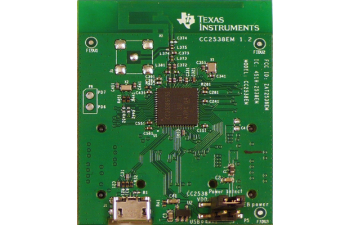
\includegraphics[width=8cm]{\rpDossier/images/cc2538.jpg}
\caption{Carte CC 2538}
\label{cc2538}
\end{figure}

Nous les avons utilisées avec une autre carte de TI, la SmartRF06 (\cref{smartrf06}), conçue pour brancher les CC 2538 pour la période de développement.
Elle est équipée de divers capteurs (boutons, capteur de luminosité, accéléromètre), de LEDs, d’un écran et d’un puce de conversion permettant de communiquer avec la carte en USB.

\begin{figure}[H]
\centering
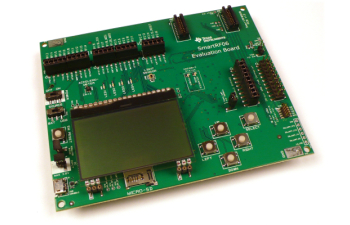
\includegraphics[width=12cm]{\rpDossier/images/smartrf06.jpg}
\caption{Carte SmartRF06 pour le développement avec une CC 2538}
\label{smartrf06}
\end{figure}

\subsubsection{Test des cartes}

\todo[Copies d’écran RF studio \& description]

\subsubsection{Programmes exemple}

\paragraph{Installation sur les cartes}

\emph{Contiki} fournit un script \emph{Python} pour installer un programme sur une carte CC 2538, appelé \emph{cc2538-bsl}, qui est intégré dans le \texttt{Makefile} \citeweb{contiki-cc2538}.
Nous avons initialement suivi les étapes décrites dans sa documentation pour configurer la communication avec les cartes CC 25358, mais le résultat a invariablement été un message d’erreur indiquant que la carte ne répondait pas aux solicitations du script (\cref{bsl-error}).

\begin{figure}[H]
\centering
\todo[Copie de l’erreur]
\caption{Erreur du script de flashage intégré}
\label{bsl-error}
\end{figure}

La lecture de la documentation de \emph{cc2538-bsl} \citeweb{bsl} ne nous a pas permis de trouver la cause du problème.
À partir des informations qui y étaient données, nous avons essayé de savoir si le \textit{bootloader} mentionné pouvait ne pas avoir été correctement configuré, grâce aux documentation de la CC 2538 \cite{cc2538-user-guide} et de la SmartRF06 \cite{smartrf06-user-guide}.
Les informations des ces documents à ce sujet étaient essentiellement similaires à celle que nous avions déjà.

Nous nous sommes alors tournés vers le logiciel développé par TI, \emph{FlashProgrammer} (\cref{flashprogrammer}).
Celui-ci ne fonctionnant que sur un système Windows, nous l’avons installé sur la machine hôte de la machine virtuelle.
\emph{FlashProgrammer} a fonctionné immédiatement, montrant que la carte n’était pas en cause.
Nous ne savons toujours pas précisément quel était le problème, mais il est très probablement localisé soit dans \emph{cc2538-bsl}, soit dans la connexion USB virtuelle établie par \emph{VirtualBox}.

Afin de transmettre facilement les fichiers compilés par \emph{Contiki}, nous avons utilisé les outils de partage de dossier proposés par \emph{VirtualBox}.
Après configuration des droits d’accès sur la machine virtuelle, la commande \texttt{cp} suffisait pour avoir les fichiers à un endroit où \emph{FlashProgrammer} pouvait aller les chercher.

\begin{figure}[H]
\centering
\todo[Copie d’écran de l’interface de flashage]
\caption{\emph{FlashProgrammer}, logiciel de flashage externe à \emph{Contiki}}
\label{flashprogrammer}
\end{figure}

\paragraph{Accès au flux standard de sortie}

La \emph{SmartRF06} permet d’accéder facilement au flux de sortie standard des programmes : les pilotes USB créent un port de communication (port \texttt{COM} sous Windows, \texttt{ttyUSB} sous Linux) utilisable avec un terminal virtuel comme \emph{PuTTY} (\cref{putty}).

\begin{figure}[H]
\centering
\todo[capture d’écran de PuTTY]
\caption{Sortie d’un programme consultée avec \emph{}PuTTY}
\label{putty}
\end{figure}

\paragraph{Manipulations des LEDs et boutons}

Nous avons commencé par tester l’exemple conçu spécifiquement pour la CC 2538, classé dans le dossier \texttt{cc2538dk}.
Ce programme utilise plusieurs fonctionnalités de la carte de développement \emph{SmartRF 06}, mais nous avons concentré notre étude sur celles utiles pour le développement de notre démonstrateur :

\begin{itemize}
	\item le programme utilise les boutons pour sélectionner la fonctionnalité à tester, que nous avons utilisé comme entrée dans notre programme de démonstration ;
	\item plusieurs des démonstrations font clignoter les LEDs, que nous avons utilisées comme sortie de notre programme de démonstration.
\end{itemize}

\paragraph{Communication UDP}

Afin de nous familiariser avec la pile réseau de \emph{Contiki}, nous avons ensuite compilé et exécuté les programmes de l’exemple classé dans le dossier \url{ipv6/simple-udp-rpl}.
Cet exemple est constitué de trois programmes qui échangent des messages en UDP sur 6LoWPAN.

Tous ces programmes envoient leurs messages à des instants aléatoires de chacun des intervales consécutifs de vingt secondes suivant le démarrage du programme, ce qui assure un temps moyen de ving secondes entre les messages.
Nous n’avons pas trouvé de documentation pour ce choix, mais on peut supposer qu’il réduit les problèmes de collisions.

\subparagraph{\textit{Broadcast}}

Ce programme peut être utilisé seul sur plusieurs cartes, qui envoient alors régulièrement des messages à l’ensemble de leurs voisins.
Chaque carte indique sur son flux de sortie standard l’envoi et la réception de messages, ce qui permet de vérifier que la connectivité est établie.

Nous avons modifié l’exemple de façon à numéroter les messages, pour vérifier que tous les messages étaient reçus.
C’est à cette occasion que nous avons rencontré le problème posé par les variables locales (voir \cref{variables-locales}) et que nous avons cherché à mieux comprendre l’architecture de \emph{Contiki}.
Cette modification nous a permis de constater qu’un nombre non négligeable de messages n’arrivaient jamais à destination.

\subparagraph{\textit{Unicast}}

Les deux programmes d’exemple en \textit{unicast}, \texttt{unicast-receiver} et \texttt{unicast-sender} sont conçus pour fonctionner ensemble : une des deux cartes a un rôle de serveur (\textit{receiver}), l’autre de client ((\textit{sender})).
Comme dans l’exemple de \textit{broadcast}, l’envoi et la réception de messages est indiquée sur le flux standard de sortie ; il sont en plus déjà numérotés.

Cette architecture serveur-client utilise un mécanisme de services intégré à \emph{Contiki} sous le nom de \emph{servreg-hack} \citeweb{servreg-hack} : ce processus se charge d’annoncer aux nœuds voisins qu’il fournit un service (identifié par un nombre entier), de retenir les services annoncés par ses voisins et de retransmettre ces annonces.
Il permet ainsi de ne pas coder en dur dans le code du programme les adresses IP, rendant possible l’évolution d’un réseau d’objets connectés sans recompilation de tous les programmes lors d’un changement dans la répartition des tâches.

\paragraph{Développement d’un programme d’action à distance}

Nous sommes repartis de ces deux exemples pour concevoir les deux programmes de démonstration suivants. Les sources du programme sont disponibles sur \emph{GitHub} à l’adresse
\begin{center}
\url{https://github.com/loicguillaume/projet}.
\end{center}

\begin{description}
	\item[\texttt{leds-slave}]
		La carte exécutant ce programme a le rôle de serveur d’affichage ; elle expose ce service grâce au mécanisme fourni par \emph{servreg-hack}.
		Lorsqu’un client la solicite, elle met à jour l’état de ses LEDs en fonction de la demande.
	\item[\texttt{leds-master}]
		La carte exécutant ce programme réagit aux actions de l’utilisateur sur ses boutons en envoyant des requêtes de modification au serveur d’affichage.
		Afin de pouvoir suivre la mise à jour des LEDs sur la carte serveur, ce programme met aussi à jour ses propres LEDs pour refléter l’état dans lequel le serveur devrait se trouver un fois à jour.
\end{description}

La carte exécutant ce dernier programme permet à l’utilisateur de modifier un à un l’état des quatre LEDs, en faisant correspondre l’appui sur un chacun quatre boutons directionels avec le changement d’état d’une des LEDs.

Nous avions dans un premier temps imaginé n’envoyer au serveur des requêtes ne contenant que les modifications à effectuer, mais comme les messages entre les cartes étaient trop souvent perdus, nous avons décidé d’envoyer un état complet à chaque mise à jour.
Plus précisément, le client envoie deux types de demandes de mises à jour (indifférenciables du point de vue du serveur) : lorsque l’utilisateur change l’état des LEDs en appuyant sur un des boutons, celui-ci est immédiatement envoyé au serveur afin que la mise à jour soit le plus rapide possible ; pour ne pas laisser le serveur dans un état incohérent trop longtemps si ce message de modification est perdu, l’état est de nouvaeu envoyé toutes les dix secondes.

Les implémentations initiales de ces deux types d’envois étaient indépendantes temporellement : les messages de rappel étaient envoyés exactement toutes les dix secondes, quelles que soient les actions de l’utilisateur.
Afin d’éviter d’encombrer la pile 6LoWPAN et le canal hertzien inutilement avec une mise à jour de rappel suivant immédiatement la mise à jour de changement, le compteur temporel des mises à jour de rappel est désormais réinitialisé systématiquement lors d’une action de l’utilisateur.
